\chapter{Architecture\ifdraft{ (Joe K./Dan) (80\%)}{}}
\label{chapter:architecture}

The \emph{architecture} of a computing system, akin to the
architecture of a purely physical artifact like a bridge or a
building, is its high-level structure. Just as when designing a
bridge, many choices must be made when designing a computing system;
these choices are driven by the system's requirements, both technical
and non-functional, as well as by external factors such as the
availability or affordability of computing hardware or network
bandwidth. In this chapter we describe the architectural issues
associated with E2EVIV systems, present a model encompassing the
various possible architectural choices for such systems, and briefly
explore some architectural variants.

It is important to note that we are \emph{not} making a concrete
recommendation for a specific E2EVIV system architecture. The
cryptographic foundations of E2EVIV protocols have been developed to a
point where we have fairly high confidence in their ability to
eventually provide the required security and auditability
properties. However, there are many open engineering issues associated
with actually building, running, and maintaining an E2EVIV system that
fulfills its requirements in the face of both routine/expected
failures and a wide range of security threats. Because of these open
engineering issues, architectural experimentation---preferably,
empirical testing of various possible architectures to determine the
most appropriate one(s) to deploy in real-world election
scenarios---is vital to actually implementing a successful E2EVIV
system.

\section{Non-Functional Requirements Forcing Architectural Factors}

Several non-functional requirements of E2EVIV systems force the
inclusion or consideration of specific architectural factors. We
consider each of these in turn.

\subsection{Abstraction}

The software in an E2EVIV system must be high assurance, and must also
undergo a certification process before it can be used in actual
elections. Thus, the software must be designed and implemented with a
level of abstraction that enables the generation of convincing
evidence for its correctness. This requires development techniques
that emphasize formal specification and verification, which divide the
software system into relatively small components with well-defined,
well-constrained interfaces. Each component can then be verified
individually with respect to its specification; moreover, component
behaviors with respect to external communication can be formally
characterized in ways that allow for verification of composed
subsystems.

\tododmz{NIST component-based certification}

\subsection{Deployment}

There is a wide spectrum of possible deployment scenarios for an
E2EVIV system, each of which leads to certain decisions about its
architecture. At one extreme, the servers for an E2EVIV system could
be hosted on a bespoke server cluster, built from the ground up
specifically for the system and housed in a facility under the
physical control of electoral authorities or their authorized
representatives. At another extreme, the servers could be hosted on a
commodity cloud computing infrastructure such as Amazon EC2 or
Microsoft Azure where electoral authorities have no physical control
over the servers. A third extreme would see the system implemented in
a purely peer-to-peer fashion, with the system's functionality
distributed among all participating computers and no
specifically-designated servers. The choice within this spectrum has
significant impact on both system availability and system security
requirements.

\tododmz{agile and devops mentality vs. certification?}

\subsection{Threats}

Mitigating the potential threats to E2EVIV systems also leads to
various architectural choices. The following are some of the threats
that need to be considered. 

\paragraph{Single point of failure.} Any single point of failure, such
as a single server that contains essential data without which the
system can no longer function, is a tempting target for
attack. Therefore, the architecture should attempt to minimize or
eliminate such failure points.

\paragraph{Easy DDoS target.} The use of a fixed IP address (or
address range) for E2EVIV system components can open the system to
denial of service attacks, limit deployment flexibility, and make it
more difficult to recover from failures. The architecture should be
chosen such that IP addresses need not be hard-coded; preferably, they
should be changeable be on-the-fly (i.e., during a live election
scenario) if necessary to protect or restore system integrity.

\paragraph{DDoS mitigation.} \todokiniry{Cloudflare restrictions? I
  know how Cloudflare works, but I'm not sure which restrictions you
  were thinking of here, and I'm not coming up with anything concise
  to say about it. -dmz} \tododmz{I only meant that services such as
  Cloudflare often have restrictions on the technologies one can use
  and the network architectures that they can protect, thus
  architectural choices can impact the means by which one can provide
  high availability. -jrk}

\paragraph{Non-standard technical foundations.}
\todokiniry{Non-typical system foundations? Not sure about what to say
  about the ``threat'' here. -dmz} \tododmz{I meant the idea of using
  an OS-less foundation like HaLVM or Mirage so as to shrink the
  TCB. -jrk}

\paragraph{Multi-party computation.} \tododmz{How might an E2EVIV
  system look that built from the ground-up using MPC?
  MPC+peer-to-peer at one extreme; }

\subsection{Distributing Trust}

The distribution of trust in an E2EVIV system is critical: if the
system is not trustworthy, the election results generated by it are
inherently suspect. 

\paragraph{Trusting the Authorities.} \tododmz{threshold
  crypto. public ceremony. physical access only via specific
  locations, systems, and time frames; public bulletin board and
  public tallying}

\paragraph{Trusting the Software.} \tododmz{code signing; digital
  forensic snapshots; self-certifying systems a la FIPS kernel work;
  proof-carrying code; open protocols with redundant implementations}

\paragraph{Trusting the Servers.} \tododmz{minimize TCB; use of public
  cloud infrastructure thereby intentionally loosing control over
  which system is used for which purpose; presumption in protocol and
  system design that no system, software, or person is to be trusted;
  full peer-to-peer robust architecture in the presence of active
  malfeasance and bad software; software independence; MPC; mobile
  root of trust}

Another potential way of distributing trust in an E2EVIV system is to
use secure multiparty computation (MPC), such that no single system
needs to be completely trusted. \todo{flesh this out}

\paragraph{Trusting the Network.} \tododmz{exclusive use of TLS;
  pinned certificates; certificate signature chains that involve not
  just a CA but also the authorities; crypto integrity,
  confidentiality, and provenance of data in the TLS pipe via custom
  crypto protocol}

\paragraph{Trusting the Voting Client.} \tododmz{client cannot be
  trusted; application certification and attestation; challenges in
  web client infrastructure v-v plethora of Javascript engines;
  Javascript JIT complexity; poor Javascript language design; tools
  like JSCert\footnote{\url{http://jscert.org/}}, Anders Moller's
  tools\footnote{\url{http://casa.au.dk/software-tools/}}, and MSR's
  CVK\footnote{\url{http://research.microsoft.com/en-us/projects/cvk/}}
  only take us a little bit of the way there; still research to do a
  la SAW for asm.js}

\paragraph{Trusting the Data.} \tododmz{data-in-transit discussed
  above; use of mainstream DB technology inappropriate given the
  integrity, confidentiality, and provenence requirements; use of
  novel systems crypto like
  CryptDB\footnote{\url{https://css.csail.mit.edu/cryptdb/}}, MPC via
  frameworks like ShareMonad, (partial) homomorphic crypto}

\paragraph{Trusting the Voter.} \tododmz{physical and digital process
  of distributing credentials to the voter; false claims from, or
  mistaken memory of, voters wrt challenging votes; inability to put
  any trust in voter to keep their client up-to-date, check SSL
  certificates, etc.}

\paragraph{Trusting the Cryptography.} \tododmz{on-paper proofs
  vs. mechanized proofs; verification of implementation against
  specification; synthesis of implementation from specification; use
  of NSA/NIST-blessed cryptography; improper sources of randomness;
  use of Intel-blessed hardware crypto}

\paragraph{Trusting the Toolchain.} Ken Thompson, in his 1984 Turing
Award lecture ``Reflections on Trusting Trust'' \cite{Thompson84},
demonstrated a fundamental problem with trust in computing systems: an
attack against the toolchain (compilers, assemblers, linkers) used to
build a system can silently, and effectively undetectably, insert a
``back door'' or other corruption into the system. If this attack is
carried out successfully, inspection of the source code for the
toolchain itself and the source code for the system will show nothing
unusual; the corrupted toolchain binary introduces the corruption when
building itself, or when building the rest of the system, and also
corrupts all the tools that can be used to analyze the system
(disassemblers, binary dump tools, etc.) such that the corruption
remains hidden. Thompson himself successfully carried out such an
attack within Bell Labs, and similar attacks have occurred ``in the
wild'' against systems such as the Delphi development environment for
Windows application; with stakes as high as controlling national
election results, it is not a stretch to believe that such attacks
would be attempted against E2EVIV systems.

There are multiple ways to mitigate the possible impact of such an
attack. One is to ensure that the system uses a diverse set of
implementations of key components, all based on the same specification
but with different source code, built with different compilers, and
preferably running on different hardware and OS platforms; corruption
of a single component, or even a small number of them, could then be
detected by the uncorrupted components, and the effort required to
corrupt the system as a whole would be much higher. Another is to
counter the possibility of Thompson-style exploits by using multiple
toolchains in the technique proposed by David A. Wheeler in his
Ph.D. thesis, ``Fully Countering Trusting Trust through Diverse
Double-Compiling'' \cite{Wheeler09}.

\subsection{Scalability}

An E2EVIV system, particularly at the national level, must be able to
handle a wide range of demand. It is human nature that many voters
will wait until the last day, or even the last hour, of a voting
period to cast their votes. Moreover, it is likely that attacks
against the system---and thus, system activity in general---will
increase in intensity as the end of a voting period approaches. Thus,
while the system may see very little sustained activity for much of an
election period, it must be able to scale to extreme levels of
activity at peak times. The architecture must take this into account,
so that the system can be dynamically deployed on more computing and
network resources as need arises. This might be done either by
utilizing public cloud resources that support elastic demand or by
using private resources that can be brought on- and offline as
required.

\subsection{Availability}

E2EVIV systems must exhibit high availability;
\autoref{chapter:required_properties} stated an explicit requirement
for 99.9\% uptime during election periods and the ability to recover
from generalized (i.e., not caused by natural disaster or malicious
attack on the system) failures in under 10 minutes, and higher
availability---including in the face of malicious attack---would be
preferable. There are a number of techniques for ensuring high
availablity of systems, including the use of services like those
provided by Cloudflare to handle traffic spikes and distributed denial
of service attacks. The system architecture should be constructed in a
way that does not foreclose the use of such techniques.

\subsection{Usability}

Usability, including accessibility for disabled voters, is of
paramount importance in an E2EVIV system. Especially for the
voter-facing parts of the system, the choice of implementation
technology may have a significant effect on usability. Essentially,
choices may need to be made between using Web technologies, which have
significant advantages in terms of reach (cross-platform, able to be
used on various sizes of device), and native applications, which tend
to exhibit richer interaction design and support more accessibility
features. The architecture might also allow for both types of
implementation, potentially at the cost of additional architectural
complexity.

\section{Architectural Feature Model}

As we have seen, there are many considerations to take into account
when making architectural decisions about an E2EVIV system. Here, we
model the various architectural dimensions, and the (possibly wide)
range of choices within each, to give a sense of the potential
solution space for a workable E2EVIV system architecture.

The Business Object Notation diagram in \autoref{figure:arch-choices}
shows the architectural choices that need to be made; for each
attribute of the architecture, a list of possible choices is
provided. There are 7 listed dimensions, three of which have 2 and
four of which have 3 possible choices, for a total of
$2^3\cdot{}3^4=648$ possible architectural variants.

\begin{figure}[t]
\begin{center}
\lstinputlisting[style=bon,frame=lines]{architecture_resources/architecture-dimensions.bon}
\end{center}
\caption{A specification of the possible variants for an E2EVIV system.}
\label{figure:arch-choices}
\end{figure}

The architectural dimensions we have identified are the following:

\begin{itemize}
\item \textbf{Distribution of Authority} \ Authority in the
  system---that is, the ``official'' set of data stored in the system
  and control over access to and manipulation of that data---can be
  centralized or distributed. Centralized authority eliminates
  concerns about data consistency, as data can only be manipulated by
  one entity, but may cause issues related to system responsiveness,
  availability, and reliability. Distributed authority eliminates a
  single point of failure at the expense of needing to ensure data
  consistency and integrity. It is also possible to implement a hybrid
  authority model, where authority is concentrated in a small set of
  entities relative to the system as a whole; this is technically
  distributed authority because it is spread across entities, but
  behaves like centralized authority from the perspective of most of
  the entities in the system.

\item \textbf{Cryptography} \ The set of cryptographic algorithms and
  protocols used to protect voter privacy and insure ballot integrity
  is a critical component in any E2EVIV system. Security
  characterizations of individual cryptographic algorithms (e.g.,
  block ciphers such as AES, standard public key cryptosystems such as
  RSA, threshold cryptosystems such as ElGamal) can be found in the
  large body of cryptography literature, and the selection of
  individual algorithms is generally a matter of picking an
  appropriate algorithm and security strength for a given
  task. However, since novel cryptographic protocols such as those
  required to implement E2EVIV systems are not widely used or studied,
  evidence must be provided for the security of any such protocols
  used in a deployed system. Such evidence can be provided in two
  basic ways: through ``paper'' proofs that are carefully checked by
  multiple experts, or, if the protocols are mechanized in a formal
  specification language, through proofs that are automatically
  generated by cryptography protocol verifiers such as ProVerif
  \cite{ProVerif}. In general, it would be preferable for all
  cryptographic protocols in the system to be mechanized, as evidence
  could be generated repeatably and easily regenerated in the event of
  minor protocol changes; however, there may be cases where this is
  impractical. Thus, the cryptographic protocols of the system may
  have ``paper'' specifications, be mechanized in a formal system, or
  some combination thereof.

\item \textbf{Evidence of Correctness} \ The development of a high
  assurance system such as an E2EVIV system proceeds from a
  specification, at some level of formality, to an implementation that
  is intended to fulfill the specification. Assurance that the
  implementation actually does fulfill the specification can generally
  be obtained in two ways. First, the implementation can be developed
  in a way such that it is mechanically tied to the specification; for
  example, code generation techniques and refinement techniques can be
  used to mechanically generate correct implementations from
  specifications. Second, the implementation can be developed ``by
  hand'' with a set of included assertions that are meant to establish
  that the specification is being faithfully implemented; these
  assertions may then be checked by code analysis tools when building
  the system, or may be automatically compiled into testing code that
  validates the assertions when running the system. In practice, while
  it is clearly desirable for as much of the implementation as
  possible to be mechanically generated from the specification, most
  high assurance systems use some combination of these two techniques.

\item \textbf{Implementation Type} \ \todokiniry{Isn't there a
    requirement that the protocols and specs be open? Given that, and
    the previous dimension, why do we have this dimension?  i.e., what
    am I missing? -dmz} Regardless of the choices made along any of
  the other dimensions, a reference for what constitutes a ``correct''
  implementation must be provided. This can come in the form of a
  ``golden im\-ple\-men\-ta\-tion''---if a given implementation
  behaves identically to the golden implementation in all
  circumstances, it is a correct implementation. Alternatively, it can
  come in the form of open protocols and specifications, whereby any
  implemention can be checked for conformance and declared correct
  based on the results of that check.

  \tododmz{I was thinking here more about the critical choices of
    platform and programming languages. The golden implementation
    aspect still holds, since one might synthesize or build such an
    implementation via a correct-by-construction approach, but that
    version will not fulfill the performance requirements, e.g. -jrk}

\item \textbf{Key Distribution Method} \ {public ceremony; threshold
    crypto; PKI vs. web-of-trust}

\item \textbf{Deployment Style} \ The E2EVIV software can be deployed
  in one of three ways: (1) servers run entirely on trusted servers
  managed by the electoral authority or its designated
  representatives, and client applications access the servers through
  well-defined, well-controlled interfaces; (2) servers run, in whole
  or in part, on public cloud infrastructure, while client applications
  still access them through well-defined interfaces; (3) the system is
  structured in a peer-to-peer fashion, where ``server'' functionality
  is distributed across all entities in the system and at least some
  of them run in an uncontrolled environment (i.e., voters'
  computers). 

\item \textbf{Client Technology} \ Implementation of the client
  software used by voters, as well as the administration software used
  by the electoral authority, can be done in two basic ways: (1)
  develop custom applications for the various hardware/OS platforms
  that will be used by voters and the electoral authority; or (2) use
  Web application technologies to develop a single Web-based
  application that will be accessible from all (reasonable)
  platforms. It is also possible to choose both implementation
  strategies for all applications (i.e., both voters and the electoral
  authority can access the system through either native applications
  or a Web application, as they choose) or make different choices for
  different applications (e.g., the voter application is implemented
  as a Web application while the electoral authority's administration
  application is implemented as a native application).

\end{itemize}

\section{Primary Architectural Variants}

Given the many dimensions of the architectural feature model, and
number of choices in each, the number of possible architectural
variants for the system is large. Here, we briefly describe a few of
the primary system variants that can be described by the feature
model. Since we are only describing them at a high level, some of the
variants described correspond to multiple possible feature selections
in the feature model (for example, they might have any of the
different types of correctness evidence or any of the different
implementation types).

\subsection{Mirrored Servers}

One possible architecture, which features centralized authority as its
primary defining characteristic, is the ``mirrored servers''
architecture depicted in \autoref{figure:arch-mirrored-servers}. The
double arrows in this diagram (and later diagrams in this chapter)
denote \emph{client} relationships (one entity making use of another's
services), while the thick double-ended arrows denote \emph{mirroring}
relationships (entities, or groups of entities, ensuring that their
states accurately reflect each other for redundancy or availability).

\begin{figure}[t]
\begin{center}
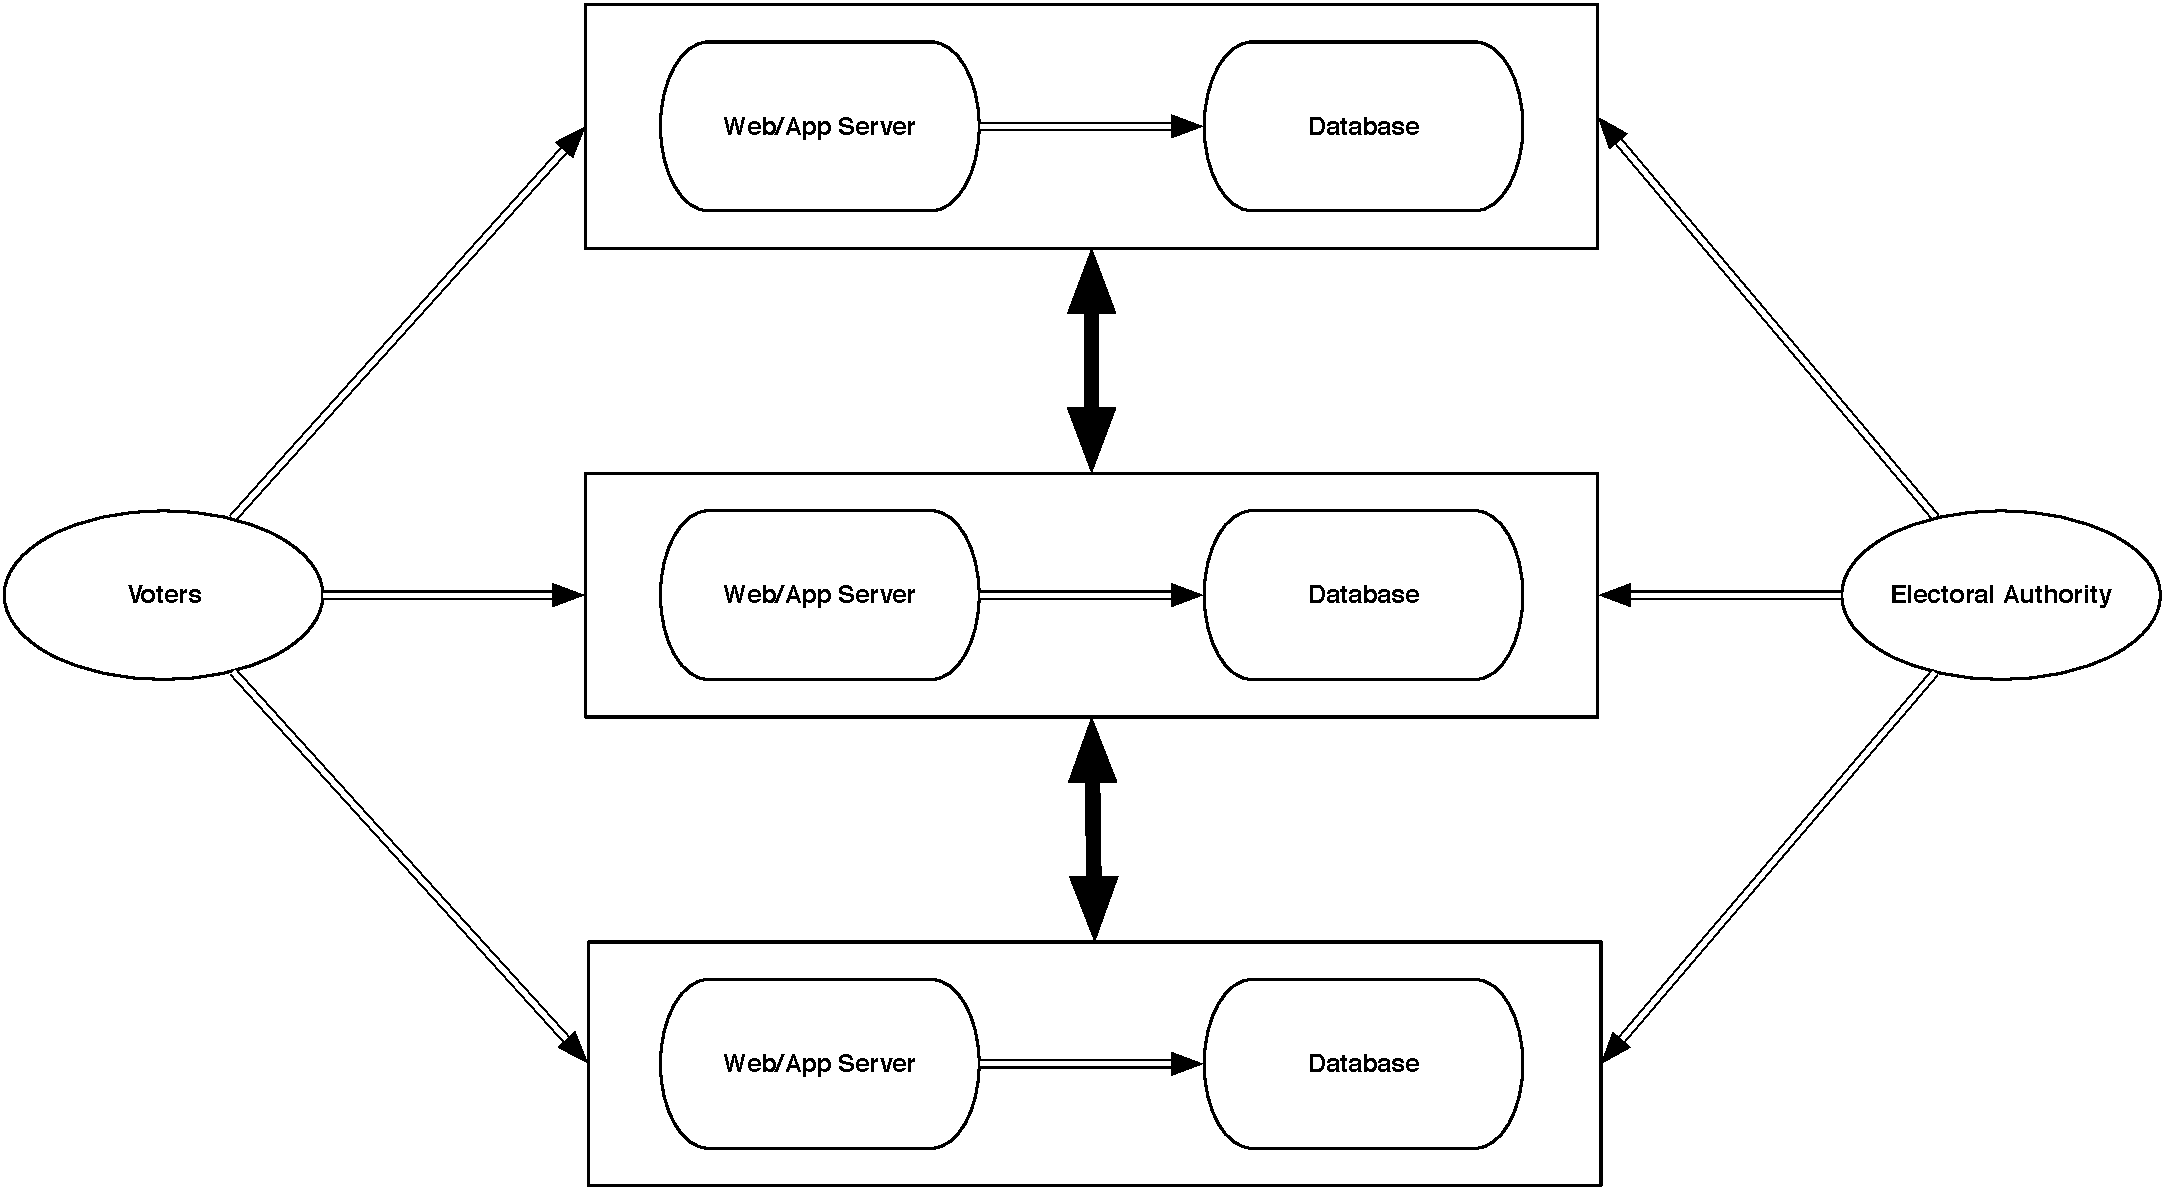
\includegraphics[width=5.5in]{architecture_resources/mirrored-servers.pdf}
\end{center}
\caption{An architecture with centralized authority and mirrored
  servers.}
\label{figure:arch-mirrored-servers}
\end{figure}

In this architecture the Web/App Server (to which voters, using either
a web-based interface or custom applications, connect to cast their
ballots) is a client of the Database, which stores all information
relevant to the operation of the E2EVIV system (ballot styles, cast
and spoiled ballots, etc.). In an actual implementation, the
monolithic Database would likely be split into multiple databases
since the access patterns and performance needs for data such as
ballot styles, cast and spoiled ballots, voter lists, etc., are likely
to be quite different. There might also be more components within each
mirror (for example, separate servers for dealing with native
applications vs. web access in a system that supports both).

Regardless of the number of servers within each mirror, the mirroring
in this architecture is done primarily for availability and
reliability; it ensures that, as long as at least one set of mirrored
servers is running, the system can remain operational (albeit perhaps
at a degraded level of responsiveness). Authority is centralized in
the sense that each mirror has a complete set of data for the system
and behaves accordingly; one mirror is designated as the
\emph{primary} mirror and is considered the authoritative source of
information in the event of inconsistency. Voters and the electoral
authority access the system by interacting with an individual
(typically, the primary) mirror, and the entire set of mirrors appears
logically as a single server-side system.

\subsection{Large Fixed Set of Servers}

Another possible architecture, which introduces the potential for
distributed authority but still has the logical presentation of a
single server-side system, is a large fixed set of servers. This
architecture, an example of which is depicted in
\autoref{figure:arch-large-fixed-set-of-servers}, still features
mirroring for redundancy and availability; however, it allows for
flexible allocation of resources. For example, there might be twice as
many Web/App Server instances as there are Database instances, or
there might be more Database instances dealing with dynamic cast and
spoiled ballot data than dealing with fixed election definition data
such as ballot styles.

\begin{figure}[p]
\begin{center}
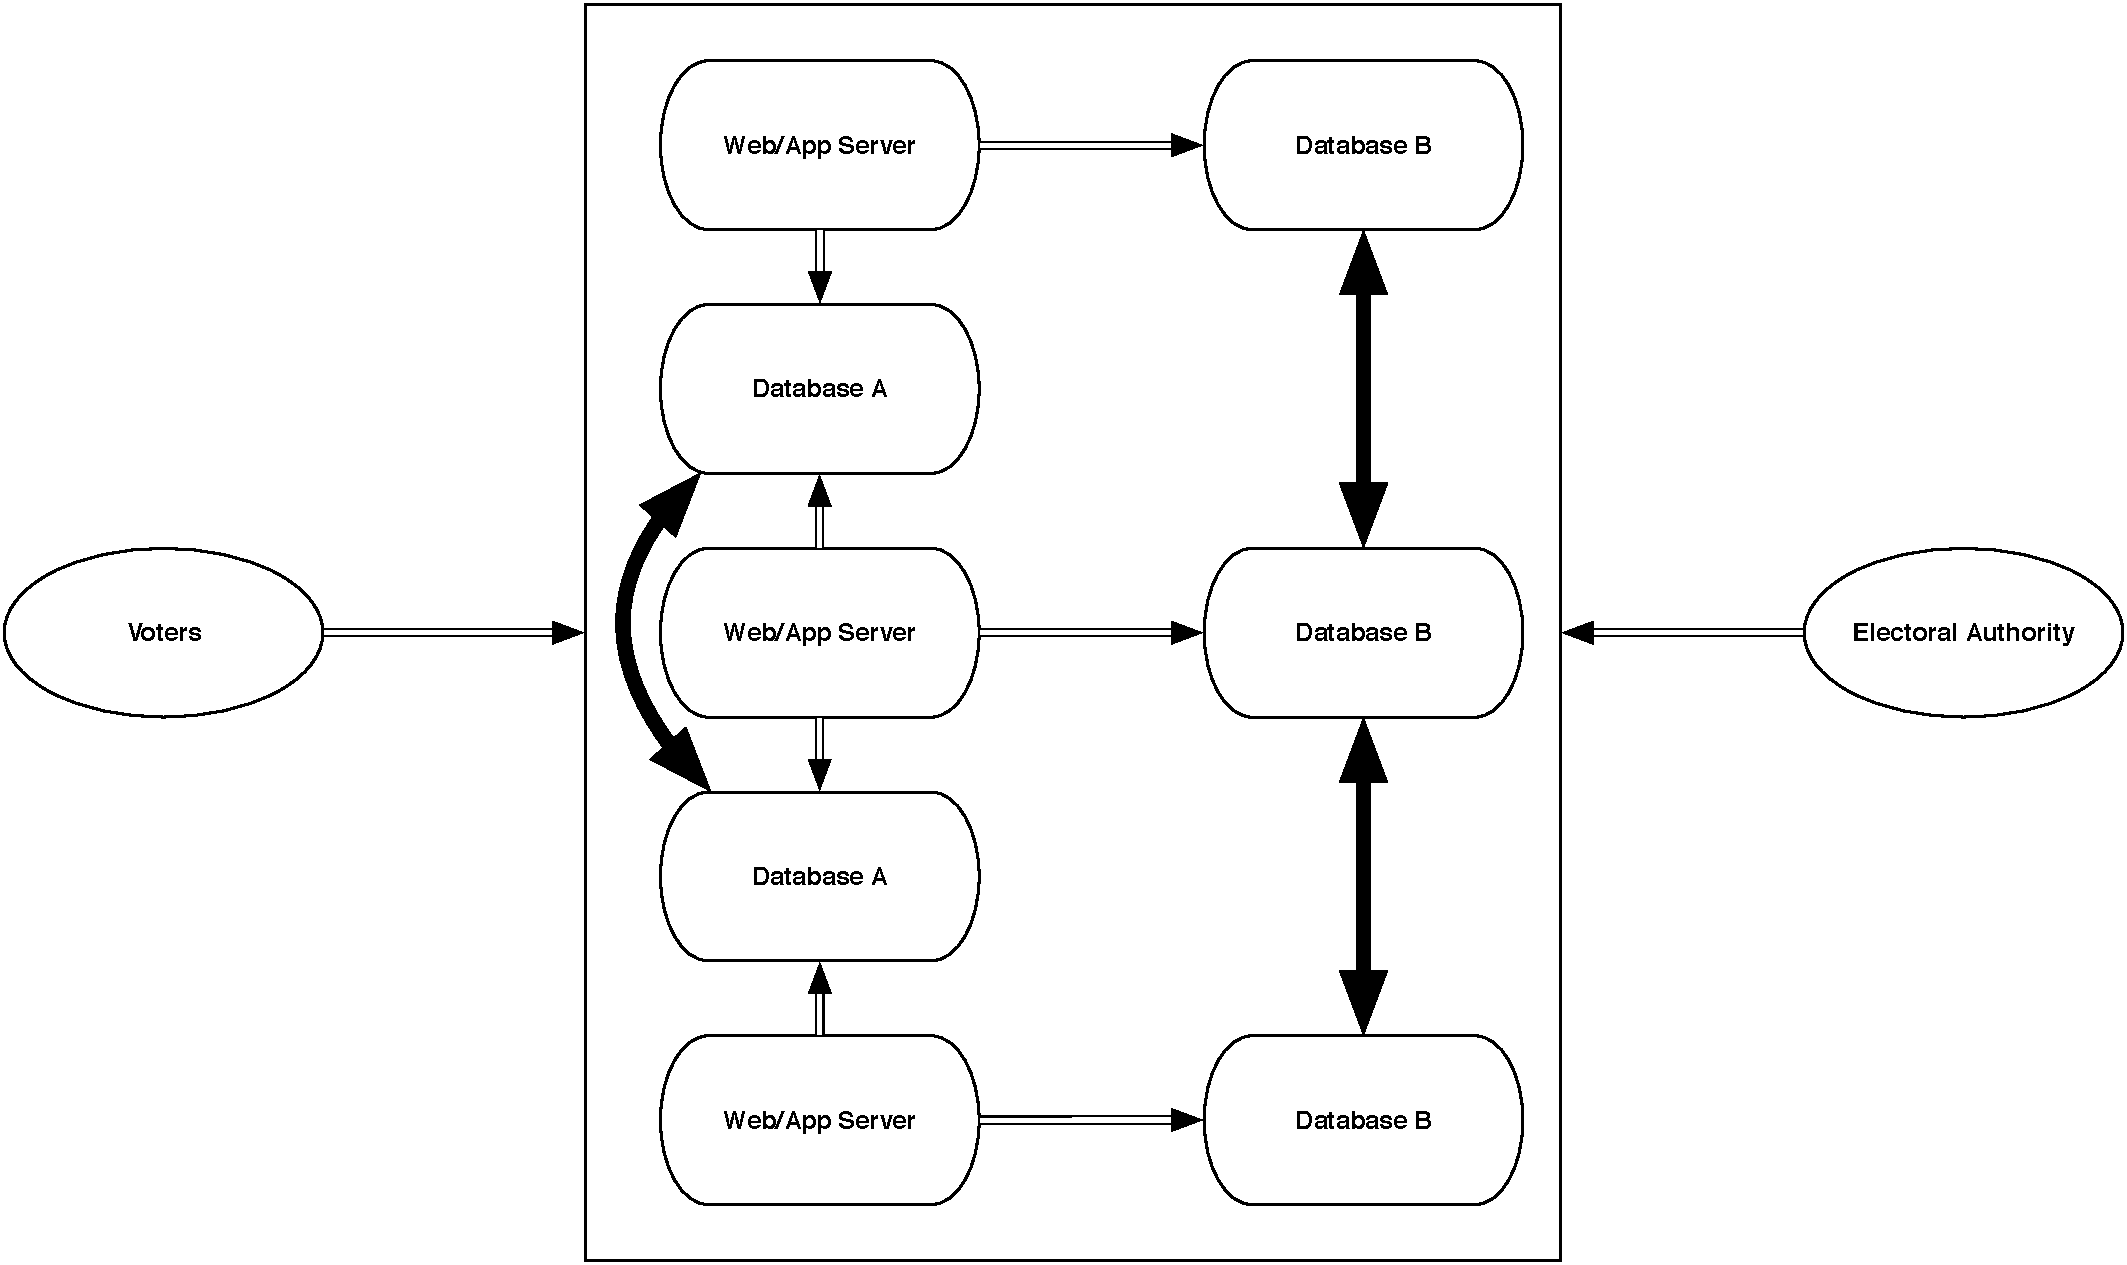
\includegraphics[width=5.5in]{architecture_resources/large-fixed-set-of-servers.pdf}
\end{center}
\caption{An architecture with a large fixed set of servers.}
\label{figure:arch-large-fixed-set-of-servers}
\end{figure}

\begin{figure}
\begin{center}
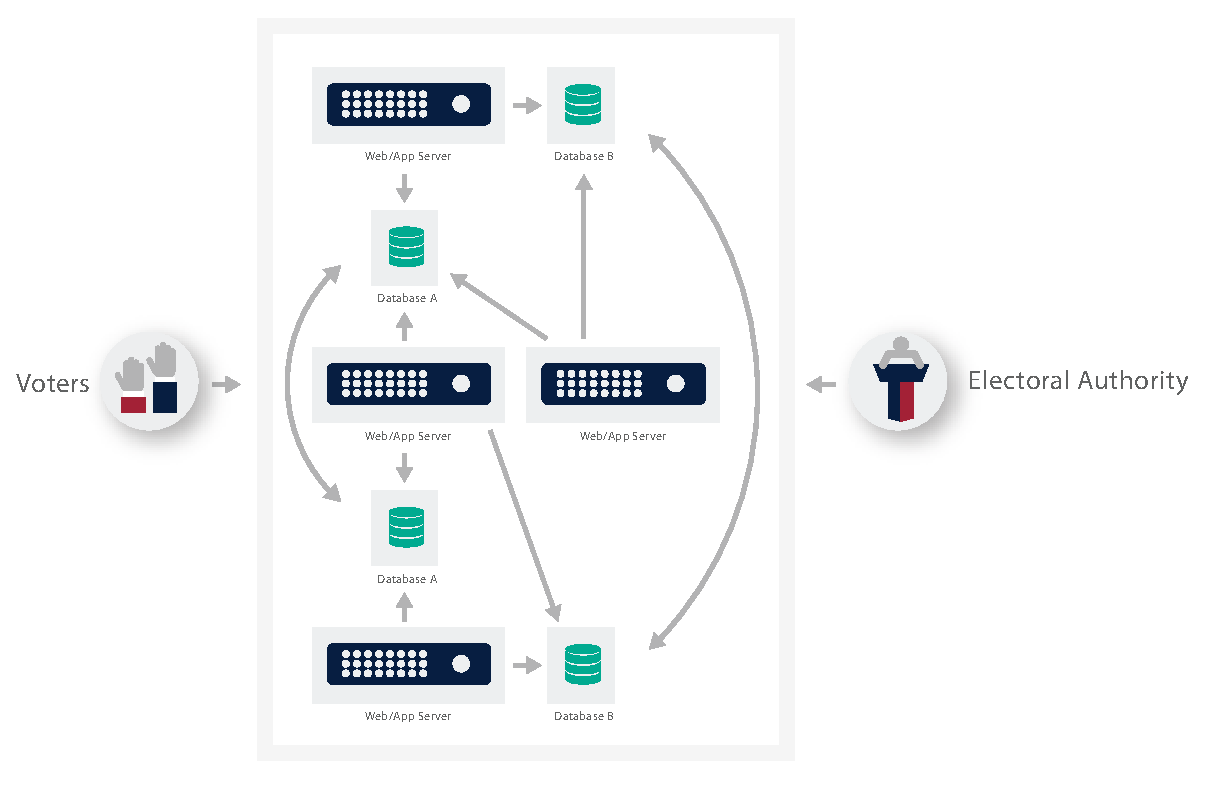
\includegraphics[width=5.5in]{architecture_resources/large-fixed-set-modified.pdf}
\end{center}
\caption{The same fixed set of servers as in
  \autoref{figure:arch-large-fixed-set-of-servers} performing a different
  allocation of tasks.}
\label{figure:arch-large-fixed-set-modified}
\end{figure}

The servers within this architecture could, amongst themselves, behave
as a peer-to-peer system, a set of client-server systems, or a set of
mirrors of various sizes for the purposes of providing high
availability and redundant storage and ensuring data consistency. A
key aspect of this architecture is that the number of servers, while
large, is fixed; this allows the topology of the servers and the
communications amongst them to be known at all times, making it
straightforward to monitor the system's health and performance and to
quickly detect any issues that arise.

As an example, \autoref{figure:arch-large-fixed-set-of-servers}---only
one of many possible server topologies in such an architecture---has
two separate mirrored Databases (one with two mirrors, and one with
three) being accessed by three separate Web/App Servers. If it is
determined that the Databases are underloaded and the Web/App Servers
are overloaded, one of the servers running Database B could easily be
repurposed to run an additional Web/App Server
(\autoref{figure:arch-large-fixed-set-modified}) without changing the
actual set of servers in the architecture and without compromising the
redundancy of data storage in the system.

While one possible deployment of this architecture would see every
server containing the full authoritative data set, it is far more
likely that each would contain only part of it and that the authority
in the system would, therefore, follow either a hybrid or a distributed
model. 

\subsection{Dynamic Cloud}

The two previous architectural variants involved the deployment of a
fixed set of servers, either as a collection of mirrors or in other
topologies. The next variant departs from these by deploying services
not across a fixed set of servers, but instead within a dynamic cloud
infrastructure, while still presenting itself as a single server-side
system for external interactions. Such an infrastructure allows for
the addition and removal of computing resources as necessary during
the operation of the system, using various distributed communication
and consistency protocols to deal with resource changes in a way that
is effectively invisible to the system's users while maintaining data
integrity and service
availability. \Autoref{figure:arch-dynamic-cloud-small,
  figure:arch-dynamic-cloud-large} show snapshots of a dynamic cloud
deployment at times when it has five and eleven running servers,
respectively. Note, in particular, that the client relationships among
the servers in the cloud may evolve over time as well; for example, in
\autoref{figure:arch-dynamic-cloud-small}, the server at the ``top''
of the cloud could establish direct communication with the server at
the ``bottom left'' of the cloud if necessary.

\begin{figure}[p]
\begin{center}
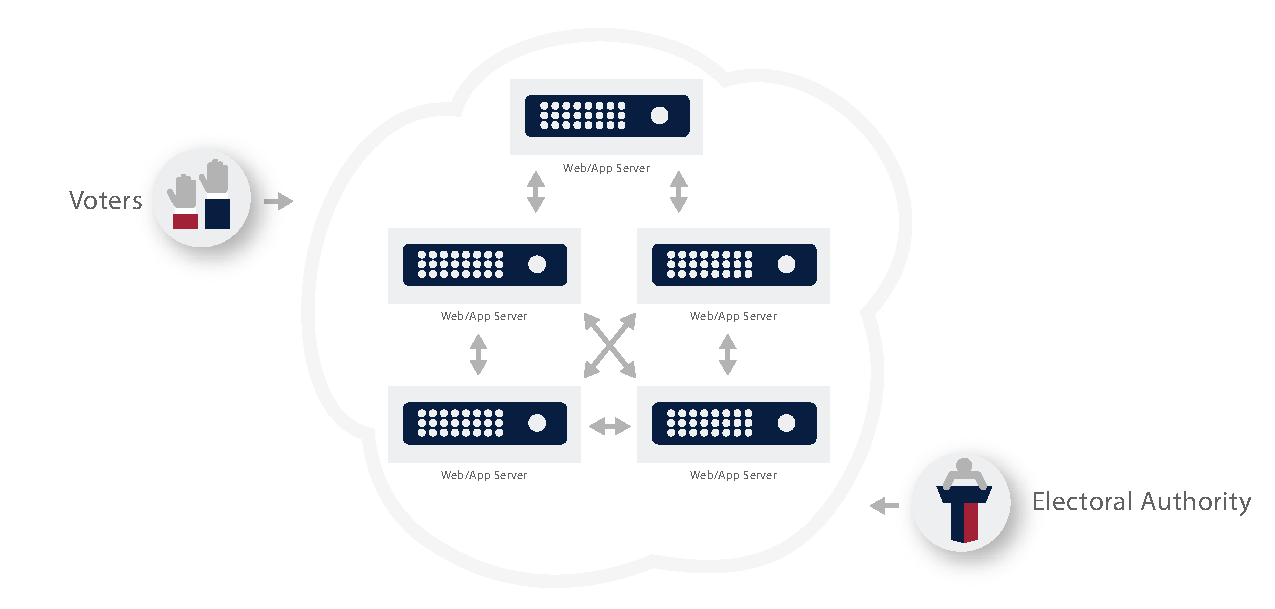
\includegraphics[width=5.5in]{architecture_resources/dynamic-cloud-small.pdf}
\end{center}
\caption{A dynamic cloud architecture with a small number of servers.}
\label{figure:arch-dynamic-cloud-small}
\end{figure}

\begin{figure}
\begin{center}
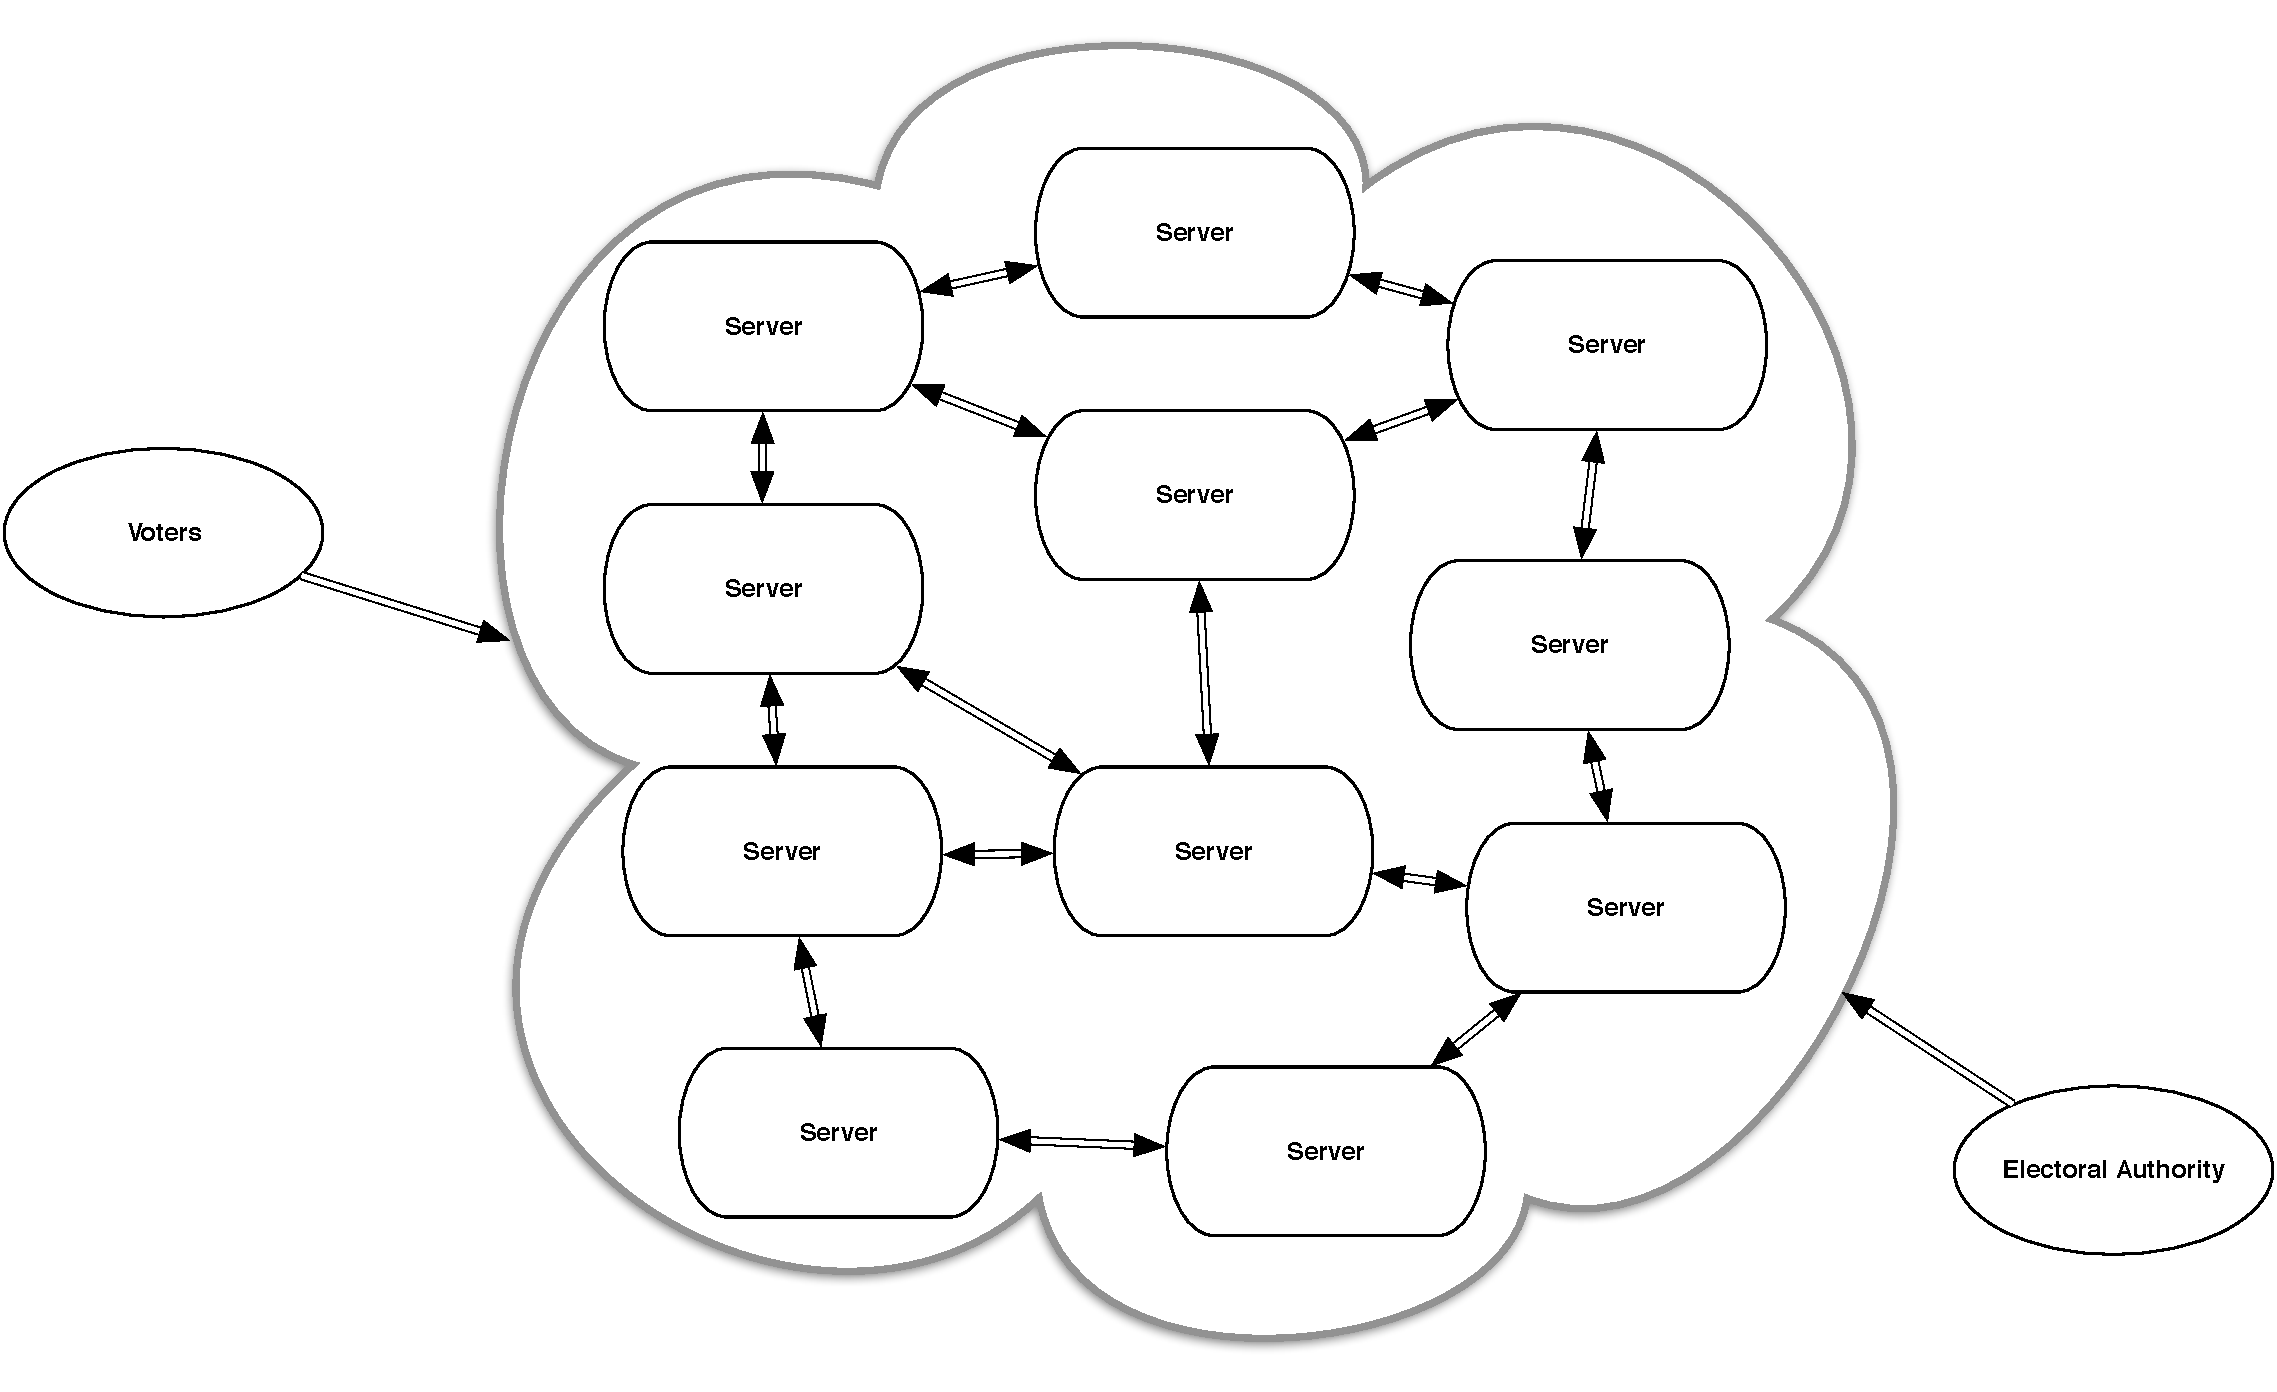
\includegraphics[width=6.5in]{architecture_resources/dynamic-cloud-large.pdf}
\end{center}
\caption{A dynamic cloud architecture with a larger number of servers.}
\label{figure:arch-dynamic-cloud-large}
\end{figure}

Effectively, a dynamic cloud deployment behaves similarly to a
deployment with a large fixed number of servers; the main difference
is that the number of servers is variable. This allows for the system
to initially consume minimal resources, expanding or contracting as
necessary (within the bounds of the dynamic cloud) to maintain
acceptable response time and availability in the face of elastic
demand.

Despite the use of the word ``cloud'', a dynamic cloud architecture
need not actually be deployed on a public cloud infrastructure;
private cloud infrastructures consisting of only trusted servers may
be built as necessary to support the system.\footnote{In the E2EVIV
  context, however, public cloud infrastructures are likely preferable
  for economic reasons; it is virtually inconceivable that an
  electoral authority or its suppliers could build a cloud
  infrastructure with scale and reliability comparable to existing
  public cloud infrastructures at reasonable cost.}  Regardless of
whether the system is deployed on a trusted or public infrastructure,
authority in a dynamic cloud architecture follows either a fully
distributed or a hybrid model; some servers in the cloud may have
authority over others, or they may interact using consensus protocols
or similar mechanisms.

\begin{figure}[t!]
\begin{center}
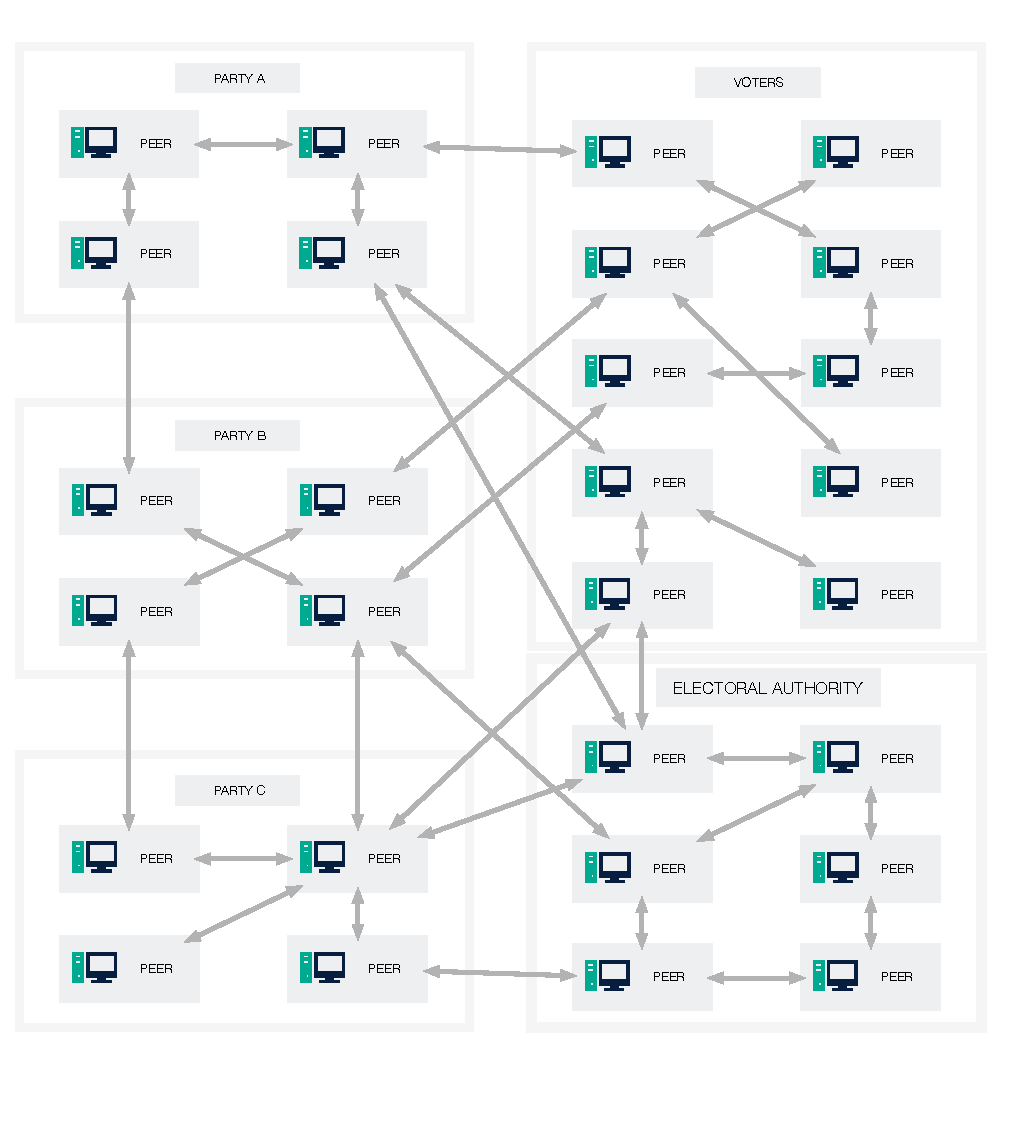
\includegraphics[width=6.5in]{architecture_resources/peer-to-peer.pdf}
\end{center}
\caption{A peer-to-peer architecture.}
\label{figure:arch-peer-to-peer}
\end{figure}

\subsection{Peer-to-Peer}

In all the architectural variants described so far, the system
presents itself as a single ``server'' regardless of its ``internal''
network topology. In a \emph{peer-to-peer} implementation, the
computational work of the system is distributed across all the
participants and there is no clearly defined distinction between
``client'' and ``server''. For example,
\autoref{figure:arch-peer-to-peer} depicts a peer-to-peer system with
a number of peers belonging to individual voters, some belonging to
political parties (A, B and C), and some belonging to the electoral
authority. The double-headed arrows in the figure represent
communication links among the peers; for example, if the upper-left
peer belonging to Party A needs to communicate with the lower-right
peer belonging to the electoral authority, it must send a message that
travels across at least 7 communication links. The communication links
in a peer-to-peer network typically change over time, based on each
peer's knowledge about its network environment and the locations of
other peers.

Authority in a peer-to-peer architecture is fully distributed. In the
case of an E2EVIV system, the electoral authority would set up and
maintain some trusted peers as a way to ``bootstrap'' the peer-to-peer
network, and political organizations (parties, lobbying groups, etc.)
might also choose to maintain peers, perhaps with their own
implementations of the election software in a system designed with
open protocols and specifications, as a way of participating in the
electoral process and strengthening trust in the results. Individual
voters running the software on their own machines would also be peers
for the duration of their voting sessions (or longer, if they chose to
contribute to the management of the election by leaving the software
running); effectively, a peer-to-peer architecture is a way of
``crowdsourcing'' the resources required to run election system. 

A peer-to-peer architecture raises significant security concerns
that differ from those of the other architectures we have
described. While some of the computer systems controlled by the
electoral authority might be trusted, the vast majority of systems
belonging to individual voters or political organzations will
certainly not be; it is impossible to run a peer-to-peer E2EVIV system
using only trusted computing resources.\footnote{This is true of pure
  peer-to-peer architectures of the type we are discussing in this
  section; an architecture where only the \emph{servers} interact in a
  peer-to-peer fashion while presenting a single interface or set of
  interfaces to clients can, as previously noted, be implemented on a
  fixed set of servers or in a dynamic cloud.} It is therefore
important to ensure that no corrupt peer, or set of corrupt peers, can
undetectably compromise election results, violate voter privacy, or
otherwise violate the E2EVIV system requirements.

One way to address this problem is to employ a \emph{blockchain}, like
that used in Bitcoin and other cryptocurrencies, to log critical
election information (cast and spoiled ballots, the fact that a given
voter has voted in the election, etc.). A blockchain is a public
write-only ledger, collectively maintained by the peers in the system,
that records a sequence of events. The mechanism by which this
recording is done ensures that the peers reach a consensus about the
events that have occurred and their ordering, and that once an event
(such as the casting of an encrypted ballot) has been placed in the
ledger it can be neither modified nor reordered with respect to other
events. As long as more than half of the peer computing power in the
network is ``honest'' and follows the correct protocol, the integrity
of the ledger is guaranteed. At any given time, it is likely that the
computing power contributed by the electoral authority and
high-profile political organizations---which can be hosted on trusted,
closely-monitored computing systems---will vastly outweigh the
computing power contributed by individual voters during their ballot
casting sessions; thus, maintaining the integrity of a blockchain
should be straightforward in an E2EVIV system. However, other aspects
of implementing a peer-to-peer architecture---such as distribution of
the computing client to voters and organizations, achieving sufficient
ease of use and performance, etc.---may prove more difficult.

\section{Summary}

As can be seen from the many architectural dimensions we have
described and the primary architectural variants we have briefly
discussed, there are many different ways in which an E2EVIV system
could be designed and implemented. It is not clear which of the
primary variants would be the ``best'' option, nor is it clear exactly
what criteria would be used to make that determination between
multiple architectures that fulfill all the E2EVIV
requirements. Further research and experimentation is therefore
necessary to determine a suitable path forward for E2EVIV
implementation and deployment.

